%!TEX root = thesis.tex
\subsection{Verteilung} % (fold)
\label{sub:verteilung}
Die Ergebnisse, die hier besprochen werden, finden sich allesamt in Anhang \ref{Anhang-Messwerte-Verteilung}. Bei der Testreihe wurde die Knotenzahl fest auf 100 000 festgelegt und der Kantengrad im Durchschnitt auf 750 gelegt. Jeder Graph hat also auch die selbe absolute Kantenzahl. Diese Zahl wurde relativ hoch angesetzt, um genug Spielraum für die Variation der Verteilung zu haben. Ein Graph, dessen minimaler und maximaler Knotengrad weit vom durchschnittlichen Knotengrad entfernt ist, wird \textit{ungleichmäßig} genannt. Das Gegenteil dazu wird als \textit{gleichmäßig} bezeichnet. 

Zunächst fällt auf, dass die seriellen Laufzeiten in der Praxis konstant sind, wie es die Theorie uns sagt. Dadurch ist in dieser Testreihe der Speedup besonders gut vergleichbar. In Abbildung \ref{fig:verteilung_speedup} ist die oberste Kurve der Speedup des gleichmäßigsten Graphen und die untere Kurve die des ungleichmäßigsten Graphen. Es ist sehr deutlich zu sehen, dass das Parallelisierungspotential eines Graphen stark von der Verteilung der Knotengrade abhängt. Um so gleichmäßiger diese verteilt sind, um so besser funktioniert die Parallelisierung. Ein mögliche Erklärung ist, dass bei einem gleichmäßig verteilten Graph die Wahrscheinlichkeit größer ist, dass die Rechenlast gleichmäßig auf alle Places verteilt wird. Bei ungleichmäßigen Graphen hingegen, ist es eher zufällig, auf welchem Place wie viele aktive Knoten liegen. Auf die Größe der Datenmengen, die zwischen den Places transportiert werden muss, dürfte die Verteilung keinen Einfluss haben.

\begin{figure}
	\centering
	\label{fig:verteilung_speedup}
	\caption{Speedup des 1D-Algorithmus über Anzahl der Places. Die Verteilung variiert. Als Referenzwert wurde jeweils der schnellste serielle Algorithmus genommen. Pro Graph ist eine Kurve eingezeichnet. Es wurden immer die schnellsten, gemessenen Werte verwendet.}
	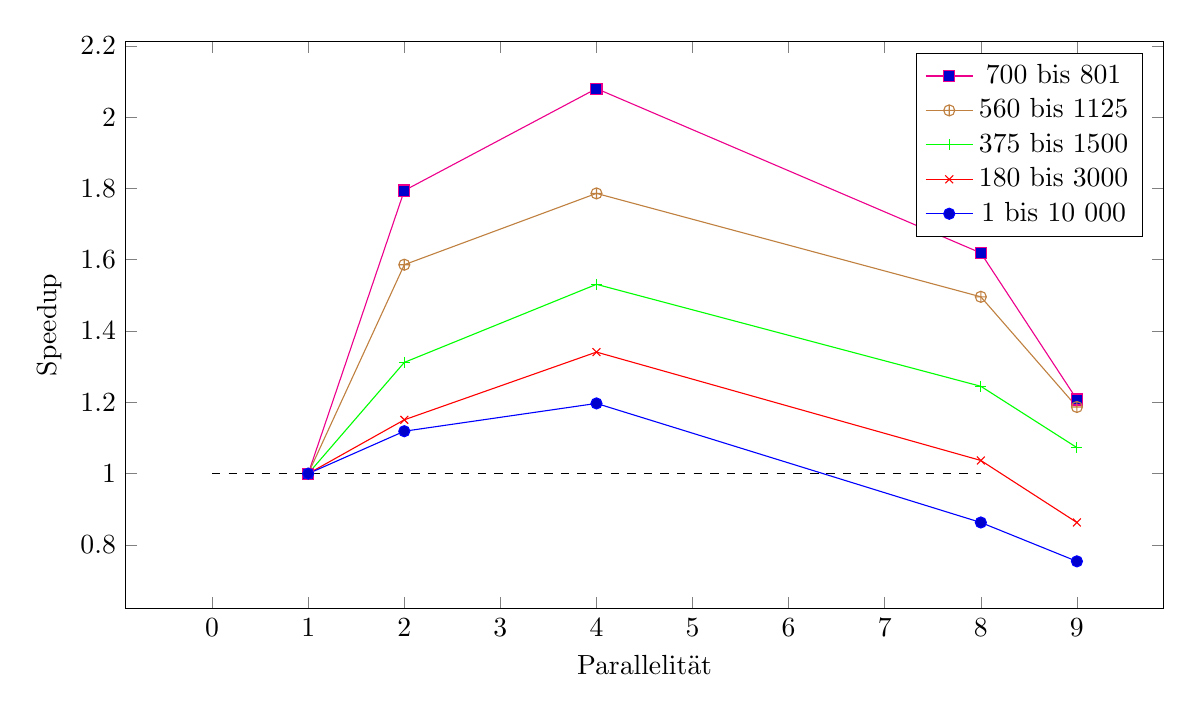
\begin{tikzpicture}
		\begin{axis}[
	        xlabel=Parallelität,
	        ylabel=Speedup,
	        width=420, height=250]

		    \addplot+[
		    magenta,
		    solid,
		    mark=square*]
		    coordinates {
		        (1,1)
		        (2,1.794)
		        (4,2.080)
		        (8,1.619)
		        (9,1.208)
		    };

		    \addlegendentry{700 bis 801}
		    \addplot+[
		    brown,
		    solid,
		    mark=oplus]
		    coordinates {
		        (1,1)
		        (2,1.586)
		        (4,1.786)
		        (8,1.496)
		        (9,1.187)
		    };
		    \addlegendentry{560 bis 1125}

		    \addplot+[
		    green,
		    solid,
		    mark=+]
		    coordinates {
		        (1,1)
		        (2,1.312)
		        (4,1.531)
		        (8,1.245)
		        (9,1.073)
		    };
		    \addlegendentry{375 bis 1500}

		    \addplot+[
		    red,
		    solid,
		    mark=x]
		    coordinates {
		        (1,1)
		        (2,1.151)
		        (4,1.341)
		        (8,1.037)
		        (9,0.863)
		    };
		    \addlegendentry{180 bis 3000}

		    \addplot+[
		    blue,
		    solid,
		    mark=*]
		    coordinates {
		        (1,1)
		        (2,1.119)
		        (4,1.197)
		        (8,0.863)
		        (9,0.754)
		    };
		    \addlegendentry{1 bis 10 000}

		    \addplot+[
		        smooth,
		        dashed,
		        black,
		        mark=none]
		    coordinates {
		    	(0,1)
		    	(8,1)
		    };

		\end{axis}
	\end{tikzpicture}
\end{figure}
% subsection verteilung (end)